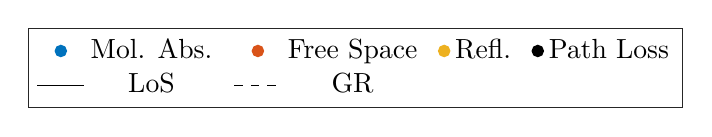
\begin{tikzpicture}

\definecolor{mycolor1}{rgb}{0.00000,0.44700,0.74100}%
\definecolor{mycolor2}{rgb}{0.85000,0.32500,0.09800}%
\definecolor{mycolor3}{rgb}{0.92900,0.69400,0.12500}%

\begin{axis}[%
width=0,
height=0,
at={(0,0)},
xmin=0,
xmax=0,
xtick={},
ymin=0,
ymax=0,
ytick={},
scale only axis,
axis background/.style={fill=white},
legend style={legend cell align=center, align=center, draw=white!15!black,at={(0,0)},anchor=center, /tikz/every even column/.append style={column sep = 0.2cm}},
legend columns = 4
]
% \addlegendimage{empty legend}
% \addlegendentry[yshift=10pt]{Frequency $f_c$ [GHz]}

\addplot [scatter, only marks, color=mycolor1, line width=0.5pt]
table{%
0	0
};
\addlegendentry{Mol. Abs.}

\addplot [scatter, only marks, color=mycolor2, line width=0.5pt]
table{%
0	0
};
\addlegendentry{Free Space}

\addplot [scatter, only marks, color=mycolor3, line width=0.5pt]
table{%
0	0
};
\addlegendentry{Refl.}

\addplot [scatter, only marks, color=black, line width=0.5pt]
table{%
0	0
};
\addlegendentry{Path Loss}

\addplot [color=black, line width=0.5pt]
table{%
0	0
};
\addlegendentry{LoS}

\addplot [color=black, dashed, line width=0.5pt]
table{%
0	0
};
\addlegendentry{GR}

% \addplot [color=mycolor7, line width=0.5pt]
% table{%
% 0	0
% };
% \addlegendentry{$181$ GHz}

\end{axis}
\end{tikzpicture}%